\chapter{Data Processing}\label{ch:2}
\epigraph{On two occasions I have been asked, ""'Pray, Mr. Babbage, if you put into the machine wrong figures, will the right answers come out?'"" ... I am not able rightly to apprehend the kind of confusion of ideas that could provoke such a question.}{Charles Babbage}

The goal of data mining can be defined as the process of obtaining knowledge from underlying data by systematic application of analytic methods to it. Applied on this thesis we are up to obtain anomalies in data and the analytic methods are the machine learning algorithms discussed in the next chapter: \ref{ch:3}. 

However, data-mining is more than applying algorithms on data. Extracting valuable results efforts among other things the consideration of a basis principle in the field of computer science known as \textit{Garbage In Garbage Out (GIGO)}. The business dictionary \footnote{http://www.businessdictionary.com/definition/garbage-in-garbage-out-GIGO.html}  defines \textit{GIGO} as an axiom used in context of computer science that signifying that no matter how sophisticated an information processing system is, the quality (accuracy, completeness, relevance, timeliness, etc) of the information coming out of it cannot be better than the quality of the information that went in. A program working on inaccurate data will only yield misleading results. The preparation of data have thus a significant contribution to the success of a data-mining goal.

There are several industry established standards like \textit{KDD, SEMMA, CRISP} \footnote{See the work of: \cite{Abraham;Ajith:2008}  for the comparison.} to name a few, invented to structure a data-mining process. The process realised in this thesis will be inclined toward to the \textit{Cross-industry process for data mining (CRISP-DM)} \cite{crisp} which is a proved data-mining process approach described in terms of an hierarchical process model.
\begin{figure}[h]
    \centering
    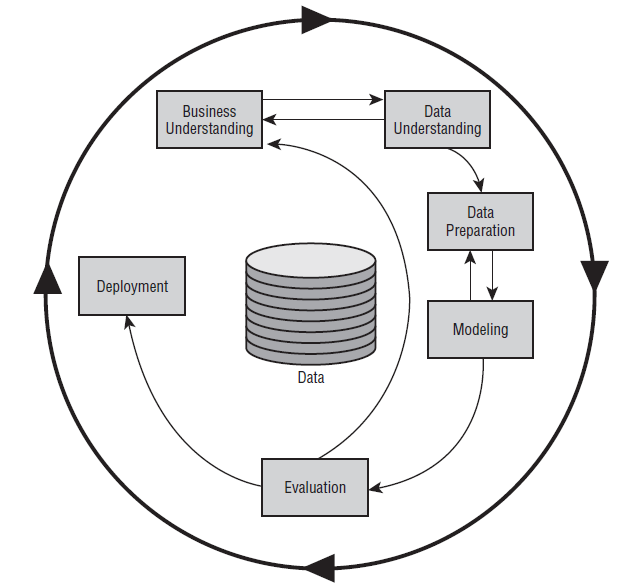
\includegraphics[scale=0.4]{Graphics/crisp-dm.png}
    \caption{CRISP-DM Process}
    \label{fig:crisp-dm}
\end{figure}
%This thesis will not adopt the complete process caused by the simple fact that a part of the methods are only for the business scope where this thesis is acting in scope of research.
\newline
\newline
\newline
This chapter will first \ref{Ch:2:Acquisition} have a macro view on the loan application process to point out the steps where our data will come from. %The goal is to have a real-world point of view on the collection process.%
Then, the first 3 phases of CHRISP-DM process are described in respect to the context of this thesis:
\begin{itemize}
    \item \textbf{Business Understanding }  
    \begin{itemize}
        \item Acquisition \ref{Ch:2:Acquisition} 
        % DATA Centered Approach, - Data driven
        \item Overview \ref{Ch:2:Overview} will discuss the macro view of the data and present insides collected by look up on it from the real-world point of view.
    \end{itemize}
    \item \textbf{Data Understanding }
        \begin{itemize}
            \item Feature Description \ref{Ch:2:FeatureDesc} provide a micro view on the available data: mention types of the features and describe the semantic.
            \item in Data Exploration \ref{Ch:2:Exploration} an  analysis of data is made by using of statistical \ref{Ch:2:SSummary} and visual \ref{Ch:2:VSummary} summary techniques, to explore data in order to bring important aspects of that data into focus. Moreover subchapter \ref{Ch:2:CorAn} expose correlated features damaging classification accuracy and data quality \ref{Ch:2:DataQuality} is dealing with inconsistent data.
        \end{itemize}
    \item \textbf{Data Preparation }
            \begin{itemize}
                \item Chapter Preprocessing \ref{Ch:2:Preprocessing} contain a composition of well researched data preparation approaches with the goal to increase the model performance. Dealing with missed/inconsistent data in \ref{Ch:2:MVI}, changing data representation to fit in the model is described in \ref{Ch:2:CTNT}. Then removing correlations \ref{Ch:2:RCF} and linear combinations \ref{Ch:2:RLCOF} in data is pointed out. As last feature normalization chapter \ref{Ch:2:FN} describe a general approach to rescale the features (give them the properties of a standard normal distribution).
        \end{itemize}
\end{itemize}

\section{Acquisition}\label{Ch:2:Acquisition}
The underlying data treated in this thesis contain information, collected during the credit enquiry process, briefly illustrated in figure \ref{fig:behav-data}. In course of the application the potential borrower provide his personal information by stepping through the application web-form. Moreover, most of the interactions with web-form elements, pressed keys or tracked time between actions is also implicitly collected. The figure \ref{fig:behav-data} show up an overview of data collecting.
The initial data used in this thesis is provided as a table. The engineering aspects regarding collecting and provisioning of the table are not part of this work and will not be discussed further. 

\begin{figure}[h]
    \centering
    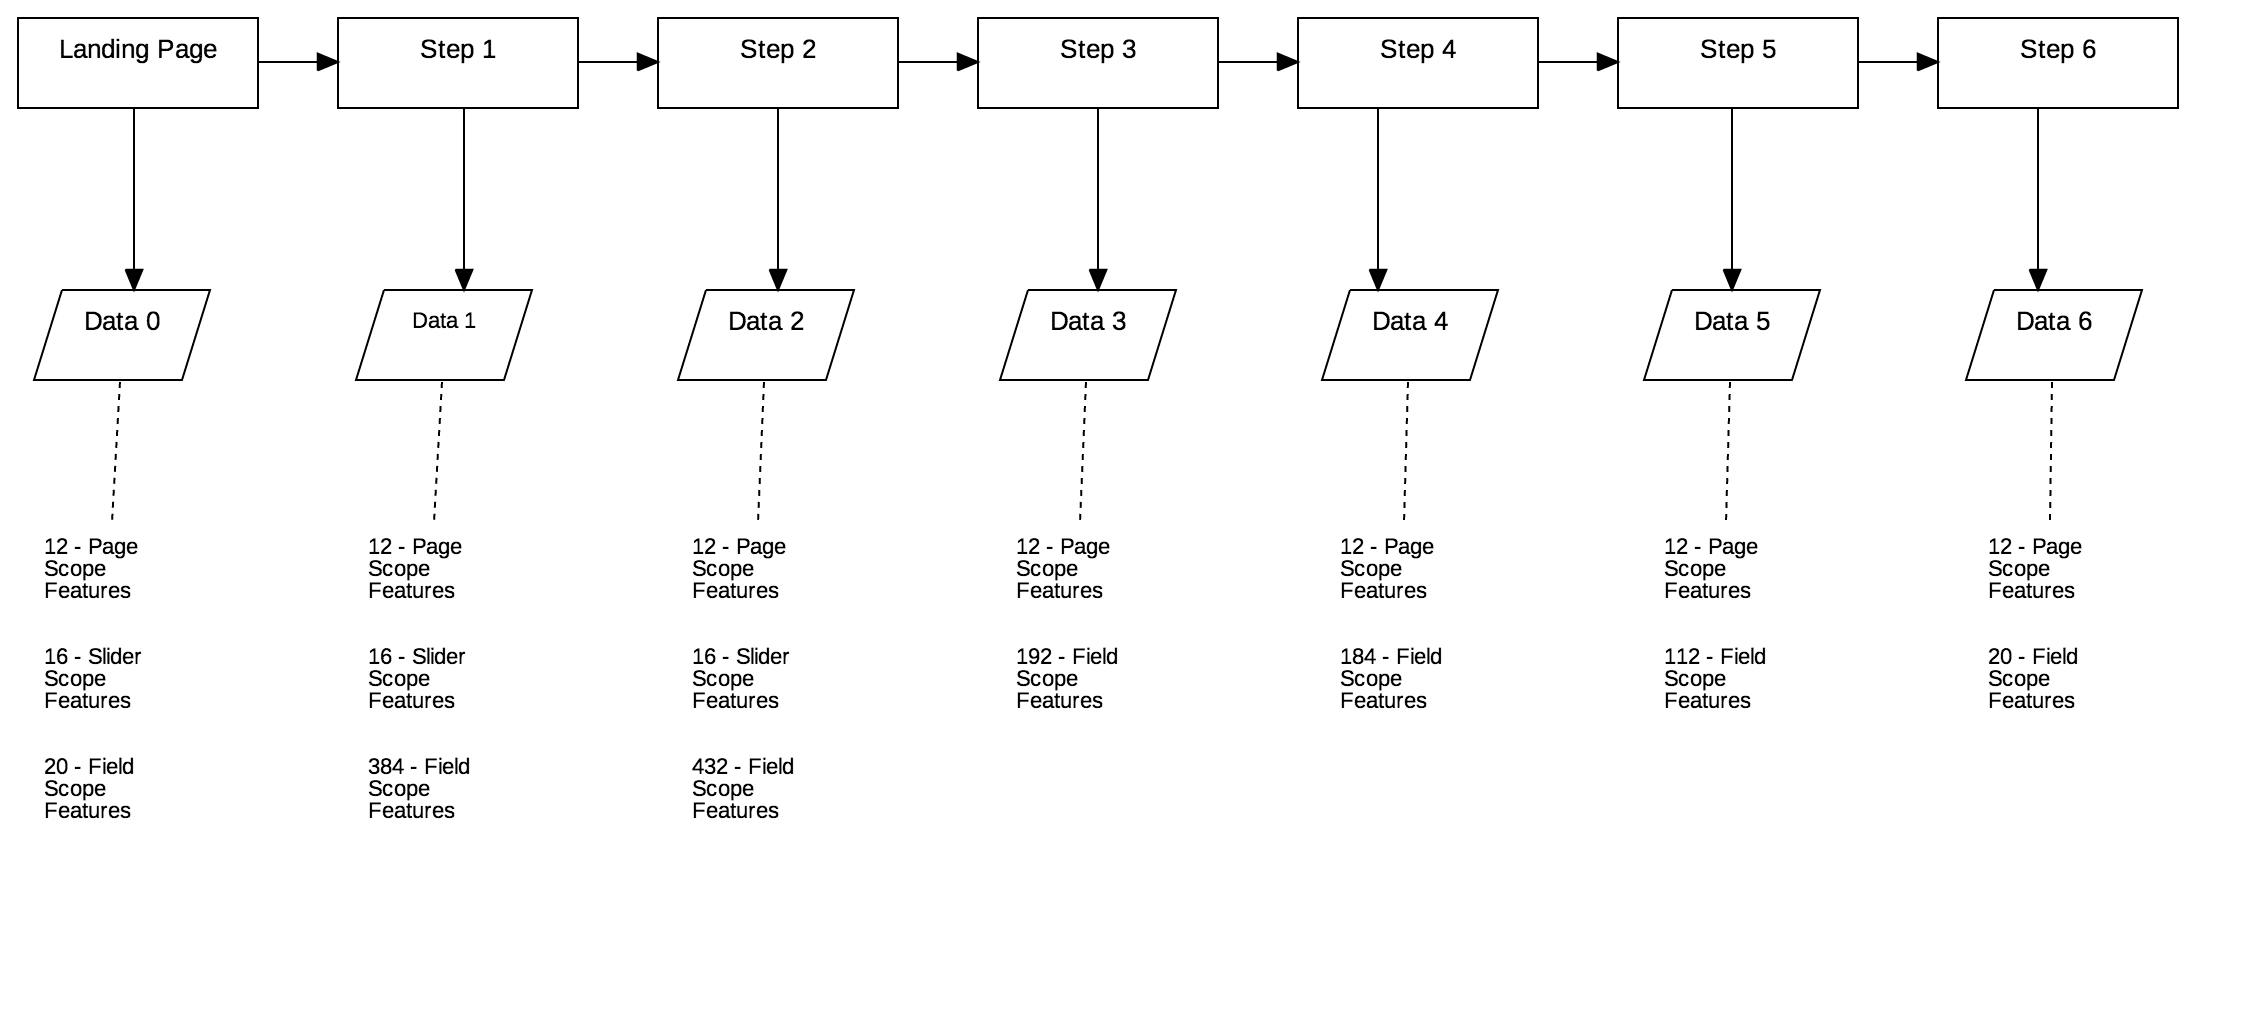
\includegraphics[scale=0.20]{Graphics/FlowchartDiagram1.png}
    \caption{Collection of Behavioral Data.}
    \label{fig:behav-data}
\end{figure}

The variables available are either categorical or numerical type and have two different sources:

\textbf{Variable Sources:}
\begin{itemize}
    \item User Input (Inputs made by the credit-applicant.)
    \item System Discovery (Variables that the application-system collect implicitly during the application-process.)
\end{itemize}

However, the variables from scope of \textit{User Input} will be excluded from further analysis based on the fact that user inputs can be malicious. Although technical barriers are implemented, it is quite usual that fraudsters try to by-pass the process by inserting malicious information to receive a loan. This leads to the logical assumption that user generated input (such as monthly income, marital status, employee status etc.) is likely to contain intentionally false information. In comparison, the system collects continuous behavioral data \textit{Discovered by System} to detect fraudulent patterns in the course of the beginning to the end of the application process. Manipulation of behavioral information is significantly more difficult than inserting alternate personal information. The most obvious obstacle for the fraudster is to identify the technique and measures of behavioral assessment and this requires both technical experience and time which is usually not in relation to the benefits (small loan sizes). Considering these aspects, the following thesis is focusing on the behavioral data rather than the user input itself. 

\subsection{Overview (business understanding)}\label{Ch:2:Overview}
An effective utilization of data in machine learning requires a good understanding of available data - also from a non technical perspective. In following this thesis will discuss real-world aspects of our underlying data that can be helpful for further work.

Each data-instance is representing information of an unique credit application, the information are historical and share the common fact that all of them are been granted. This assortment is desirable. Granted means that this applications is been approved by the scoring algorithm and issued to the borrower. Identifying anomalies signifying malicious actions in this type of data is more important to prevent fraud in the future and have thus a measurable impact on business.

In following this Thesis introduce three assumptions to semantically structure (label) the available data for further algorithmic analysis.

\textbf{Fraud:} 
A small subset contain applications that in retrospect turned out to had fraudulent intention. This can have different causes, some of them was reported by the local law enforcements, others are results of identity abuse or other malicious actions. In following, this thesis will not amplify the fraud causes in detail and outline them simple as -  fraud.

\textbf{Non Fraud:} 
Another assumption this thesis will follow is that a borrower who payed at least one installment back, had initially no fraudulent intentions. 

\textbf{Unlabeled:}
An significant subset of underlying data contain data instances not labeled as fraud but also without positive cash flow (which can possibly follow in the future), anyway, following the labeling assumptions in this thesis this data cant be either classified as fraud or non fraud, rather it can be both.

\subsection{Feature Description}\label{Ch:2:FeatureDesc}
The underlying data-set contain in total 1804 features for each instance. All features are behavioral information  been collected during the credit application process, see: \ref{fig:behav-data} to get an brief overview. Describing each feature isolated, for a such large amount of them available is unpractical. Thus a more consolidated analysis is required. Table \ref{tab:feature-summary} summarize the data types contained in our data.

\begin{table}[h!]
  \begin{center}
    \caption{Feature type summary}
    \label{tab:feature-summary}
    \begin{tabular}{c|c|c}
    Type & Amount & Rate \\
      \hline
     Categorical & 196 & ~11\% \\ 
     \hline
     Logical & 90 &  ~5\% \\
     \hline
     Numeric & 1519 &  ~84\% \\
     \hline
    \end{tabular}
  \end{center}
\end{table}

Regarding to the figure \ref{fig:behav-data} there are 3 different scopes of behavioural features.

\begin{itemize}
    %write page on step chart
    \item \textbf{Page Scope:} Variables describing behavior in the scope of one of the 7 pages must be passed in credit application process. 
    \item \textbf{Slider Scope: } Variables in scope of an web-form element called \textit{slider}, it representing two interactive bars responsible for the adjusting of the loan amount the borrower apply for and the duration till the first installment.
    % rename to element scope
    \item \textbf{Field Scope:} Is the scope of all web form elements available through the enquiry process (input fields, buttons, check boxes, etc.).
\end{itemize}


Numerical features dominating the type distribution, most of them contain behavior information e.g (count of keys been pressed by user, time between interactions on input fields, etc.), the categorical features are standing for types of web form elements triggered by user e.g (input field with text, drop down box with numbers, etc.), as last the logical fields contain boolean (TRUE/FALSE) answers on questions regarding the behavior during the application e.g (did the user read the terms of agreement?, did the user submitted his real email address on the first try?, etc.)

\section{Exploration}\label{Ch:2:Exploration}

This task addresses data mining questions using querying, visualization, and reporting techniques. These include distribution of key attributes (for example, the target attribute of a prediction task) relationships between pairs or small numbers of attributes, results of simple aggregations, properties of significant sub-populations, and simple statistical analyses. These analyses may directly address the data mining goals, they may also contribute to or refine the data description and quality reports, and feed into the transformation and other data preparation steps needed for further analysis \cite{crisp} .

\subsection{Statistical Summary of Data}\label{Ch:2:SSummary}

In total, our underlying data-set holds 95951 instances of individual applications.

According to the semantic labeling \ref{Ch:2:Overview} Table \ref{tab:instance-summary} summarize the amount of particular labels.

\begin{table}[h!]
  \begin{center}
    \caption{Instance Type Summary}
    \label{tab:instance-summary}
    \begin{tabular}{c|c|c}
    Label & Amount & Rate \\
      \hline
     Fraud & 744 & ~1\% \\ 
     \hline
     Nonfraud & 82525 &  ~86\% \\
     \hline
     Unlabeled & 12682 &  ~13\% \\
     \hline
    \end{tabular}
  \end{center}
\end{table}
It show up that non fraudulent instances clearly dominating the class membership where in the contrary the fraudulent representing a small subset. However, anomalies are rare by definition so this is a common pattern.

Summarizing over the category amount in categorical type features show up: 
\begin{itemize}
    \item \textbf{Min: } 2 Categories
    \item \textbf{Max: } 6 Categories
    \item \textbf{Mean:} 3 Categories
\end{itemize}
This observation is important insofar as each category adds an further dimension during the categorical to numerical transformation process \ref{Ch:2:CTNT}.
There are numerous well known exploration techniques (like mathematical average, standard deviation or variance to name a few), unfortunately applying these on the high amount of features available would not necessary yield an valuable result. Based on this fact, further summary techniques are beyond the scopes and will not be considered.
\subsection{Visual Summary of Data}\label{Ch:2:VSummary} 

- Here  1-2 histograms of interesting variables, then explain that the complexity to show up everything is to high.

\subsection{Correlation Analysis}\label{Ch:2:CorAn}  /* Correlation Plot and description */

\subsection{Data Quality (missing values)}\label{Ch:2:DataQuality}
Lacks or missing of data in given data set is a common obstacle in the fields statistics and data mining. Investigation the quality of data aims to identify lacks, which should be treated - to satisfy the selected machine learning algorithm. 

According to \cite{Allison:2007} there are three categories of missing data:

 \begin{itemize}
    \item \textbf{Missing Completely At Random (MCAR)} means that the probability of missing is unrelated to the variable itself or other variables. 
    \item \textbf{Missing At Random (MAR)} address missing in variables that is unrelated to itself. For example the probability of missing in income may depends on the employment status, but not depend on the income.
    \item \textbf{Not Missing At Random (NMAR)} eventuates if the constraints of MAR are gone be violated, ergo the probability of the missing depend on the particular value.
 \end{itemize} 
 

An also important discovery made by inspecting our data is that variables which are discovered by system are sometimes lack in the data. This can be caused by different factors:
    \begin{itemize}
        \item The credit application process was executed by a non human but so called script/bot \footnote{A bot (short for "robot") is a program that operates as an agent for a user or another program or simulates a human activity on the Internet. (http://searchsoa.techtarget.com/definition/bot)}. A bot obviously skip the most of the interactions a human would have to do during the application. 
    
        \item The particular operation system on top the application is executed can be modified to block the gathering of information by the application system.
        
        \item Thus the behaviour data is describing several interactions with web-form components, some of them are optional.
    \end{itemize}
    The general notion made by this observations is \textit{missed     information - is also information} this means that important information can be extracted from lack of information.

\section{Preprocessing}\label{Ch:2:Preprocessing}
Based on the observations obtained through acquisition and exploration of our data, this section will explain the explicit steps of data transformation made in our model.

\subsection{Missing Value Imputation}\label{Ch:2:MVI} 
  - We remove all zero variance

\subsection{Removing Near Zero Variance Features}\label{Ch:2:RNZVF}

\subsection{Categorical to Numeric Transformation }\label{Ch:2:CTNT}
\subsection{Removing correlated Features } \label{Ch:2:RCF}
Correlations are noise and increase computation time
\subsection{Removing linear Combinations of Features}\label{Ch:2:RLCOF} /* Missing values where? */
\subsection{Feature Normalization}\label{Ch:2:FN} /* Missing values where? */

% FAZIIIIIIT!!!!! Data QUality kann mehr werden